\chapter{Atom-Cavity platform}

The system uses a single $^{87}\text{Rb}$ coupled to a birefringent Fabry-Perot cavity inside an ultra-high vacuum (UHV) chamber. The smaller optical beam path used for the realization of the atom-photon gate is part of a much larger setup. The full setup, named \textit{CavityX}, consists of two Fabry-Perot cavities arranged in an X formation. For the atom-photon gate, parts of the setup like the magneto-optical trap, the 850 nm red-detuned trap laser, and the microwave antennas integrated into the UHV chamber are crucial. Other components, most notably the second cavity, are not within the scope of this thesis, but will be discussed in the outlook.

\section{Cavity system}\label{sec:cavity_system}

At the heart of the CavityX system are the two crossed fiber cavities which are named the "short" cavity (SC) and the "long" cavity (LC), which differ in length ($\SI{79}{\mu\metre}$ vs. $\SI{161}{\mu\metre}$), and in the fact that the short cavity is birefringent. Each cavity fiber is held in place by an in-house built holder shown in figure \ref{fig:cavities_setup}.

\begin{figure}[h]
	\centering
	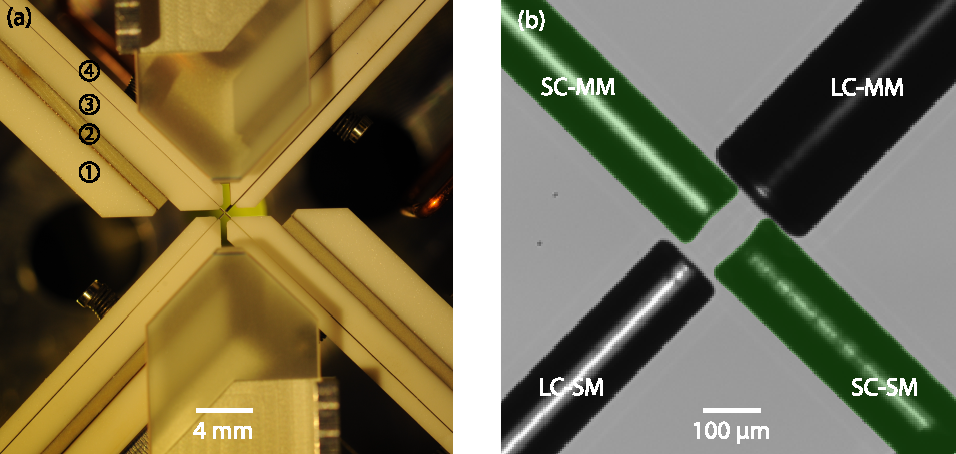
\includegraphics[width=\linewidth]{Figures/3_setup/cavities-setup.pdf}
	\caption{ vertical top view of the construction holding the crossed fiber cavities in place.
		The holder of each fiber consists of 4 elements, each of which is labeled in the picture: $\Circled{1}$ Base
		element for mounting the fiber holder to downstream components; $\Circled{2}$ Shear piezo actuator for
		active stabilization of the resonator length; $\Circled{3}$ Mount in which a V-groove is fabricated - where
		the fiber is positioned and mechanically clamped; $\Circled{4}$ Lid to clamp the fiber within the V-groove
		mount. A zoom of the center of the picture is shown in (b). The orange-colored cavity has a
		length of 161 μm and it is composed of a single-mode fiber (LC-SM) with a low reflective mirror
		coating and a multi-mode fiber (LC-MM) with a highly reflective mirror coating. The green-colored
		cavity is 75.7 μm long and is composed of a single- (SC-SM) and multi- (SC-MM) mode fiber with
		reflective coatings analogous to LC-SM and LC-MM, respectively. This photo has been colored in
		post-production.\cite{GianvitoC2026}}
	\label{fig:cavities_setup}
\end{figure}

The incoming light is coupled in and out via the single-mode (SM) fiber for either of the cavities. In order to ensure that most of the coupled light exits through the SM fiber, different mirror coatings are used for the fiber surfaces. The multi-mode (MM) fiber surfaces are coated with a highly reflected dielectric coating, while the opposing SM fiber has a dielectric coating with a lower reflectivity (\SI{10}{ppm} transmission vs. \SI{340}{ppm} transmission). This asymmetric design ensures the cavity is single-sided, causing most of the coupled-in light to then exit the cavity through the same fiber through which it entered the system.\cite{GianvitoC2026}

The cavity fibers are fabricated using a $\text{CO}_2$ laser machining technique by Manuel Brekenfeld in \cite{ManuelBThesis2023}. Changing the beam profile of the $\text{CO}_2$ laser allows for the fabrication of either spherical or elliptical surfaces, as is the case for the short cavity. This leads to a cavity mode splitting, i.e., cavity birefringence, as shown in figure \ref{fig:cavity_transmission_profiles} \\

\begin{figure}[h]
	\centering
	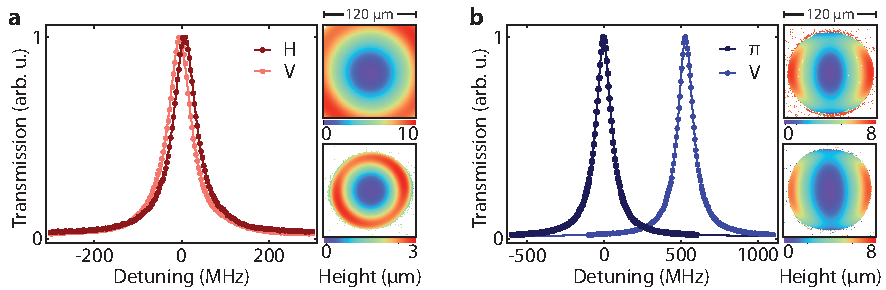
\includegraphics[width=\linewidth]{Figures/3_setup/transmission_profiles_lc_and_kc.pdf}
	\caption{Transmission spectra were recorded for both the long (a) and short (b) cavity. For
		the long cavity, the probe field was polarized to match the cavity eigenmodes, revealing a small
		residual polarization mode splitting. Contour images of the mirrors – for the MM and SM fibers –
		are shown alongside the spectrum. In contrast, the short cavity exhibited a large polarization mode
		splitting, a result of the strong ellipticity of its mirror surfaces. The error bars are smaller than the
		data point markers.\cite{GianvitoC2026}}
	\label{fig:cavity_transmission_profiles}
\end{figure}

\begin{table}[ht]
	\centering
	\begin{tabular}{l|c|c}
		\hline\hline
		Parameter                                         & Long Cavity             & Short Cavity                  \\
		\hline
		Radius of curvature of OC$_1$                     & $340\,\mu$m             & $115\,\mu$m and $283\,\mu$m   \\
		Radius of curvature of HR$_2$                     & $170\,\mu$m             & $96\,\mu$m and $167\,\mu$m    \\
		Cavity length                                     & $161\,\mu$m             & $75.7\,\mu$m                  \\
		Free spectral range                               & $0.93061\,$THz          & $1.98043\,$THz                \\
		Waist radius                                      & $3.5\,\mu$m             & $3.5\,\mu$m and $4.4\,\mu$m   \\
		Waist radius pos.\ from OC                        & $7.7\,\mu$m             & $25.8\,\mu$m and $22.7\,\mu$m \\
		Mode waist at OC                                  & $3.6\,\mu$m             & $3.9\,\mu$m and $4.6\,\mu$m   \\
		Mode waist at HR                                  & $11.3\,\mu$m            & $5.9\,\mu$m and $5.2\,\mu$m   \\
		Mode waist at cavity center                       & $6.2\,\mu$m             & $3.5\,\mu$m and $4.4\,\mu$m   \\
		Mode volume ($\lambda = 780\,$nm)                 & $10200 \cdot \lambda^3$ & $1900 \cdot \lambda^3$        \\
		Mode matching                                     &                         & 0.873                         \\
		$g(1' \leftrightarrow 2)/(2\pi)$ at cavity center &                         & 26 MHz                        \\
		Transmission through OC                           & $340\,$ppm              & $340\,$ppm                    \\
		Transmission through HR                           & $10\,$ppm               & $10\,$ppm                     \\
		Parasitic losses                                  & $80\,$ppm               & $50\,$ppm                     \\
		Total losses                                      & $430\,$ppm              & $400\,$ppm                    \\
		$\kappa/(2\pi)$                                   &                         & 58 MHz                        \\
		Linewidth                                         &                         & 116 MHz                       \\
		Finesse                                           & $14089$                 & $16531$                       \\
		Outcoupling ratio $\kappa_{oc}/\kappa$            &                         & 0.85                          \\
		Eigenmodes freq.\ splitting                       & $16\,$MHz               & $505.0(5)\,$MHz               \\
		\hline\hline
	\end{tabular}
	\caption{Cavity parameters.}
	\label{tab:cavity_parameters}
\end{table}

\section{Trapping of a Single Atom}

\subsection{Magneto-optical trap}

In order to realize an atom-photon quantum gate, one is required to have an atom trapped inside the cavity with which the photon can then interact. Therefore one needs to properly position the atom and keep it trapped at the position where it most efficiently couples to the cavity to ensure the most efficient gate operation.  \\

The starting point for this is the trapping of an atomic cloud via a magneto-optical trap (MOT). Once the atomic cloud is trapped, one turns off the MOT, causing the atoms to fall down due to the gravitational force, from which single atoms can then be loaded into the cavity's center. The concepts of a MOT are explained in \cite{AtomicPhysicsJFoot2004}.

In order to trap atomic clouds via a MOT, one needs to generate a rubidium vapor inside the UHV chamber. This is done via light-induced atom desorption (LIAD), in which atoms are dispensed from a rubidium dispenser that is placed inside of the vacuum chamber. The light source is a UV diode ILH-XQ01-S410 with an emitting wavelength of 410nm, which is pulsed for the length of time needed to load the MOT. \\

The MOT loading procedure can be divided into two phases:
First comes the loading phase in which the MOT coils, the MOT beams (a cooling laser and a repumper laser), and the UV light are switched on simultaneously. This then creates the atomic cloud and cools it down to near the Doppler temperature of \SI{146}{\mu K} for the $^{87}\text{Rb}$ $D_2\text{-line}$. \cite{SteckRb87}

Next an optical molasses is applied, which aims at bringing the atom to a temperature much below the Doppler limit. Here the detuning of the MOT beams is increased, while the optical power is decreased.

At the end of the MOT cycle, the MOT coils, beams and the UV light are switched off.

\begin{table}[ht]
	\centering
	\caption{Parameters used for the MOT loading phase.}
	\label{tab:mot_parameters}
	\begin{tabular}{@{}lr@{}}
		\toprule
		MOT coil current                                                                 & \SI{23.5}{A}                    \\
		UV diode current                                                                 & \SI{140}{mA}                    \\
		MOT beams' diameter                                                              & \SI{12}{mm}                     \\ \midrule
		\multicolumn{2}{c}{\textbf{Loading phase}}                                                                         \\ \midrule
		Duration                                                                         & \SI{1}{s}                       \\
		Cooling laser detuning from $5S_{1/2}, F = 2 \leftrightarrow 5P_{3/2}, F' = 3$   & \notetome{check detuning again} \\
		Repumping laser detuning from $5S_{1/2}, F = 1 \leftrightarrow 5P_{3/2}, F' = 2$ & \SI{0}{MHz}                     \\
		Cooling laser power                                                              & \SI{20}{mW}                     \\
		Repumping laser power                                                            & \SI{250}{\mu\watt}              \\ \midrule
		\multicolumn{2}{c}{\textbf{Molasses phase}}                                                                        \\ \midrule
		Duration                                                                         & \SI{1}{ms}                      \\
		Cooling laser detuning from $5S_{1/2}, F = 2 \leftrightarrow 5P_{3/2}, F' = 3$   & \SI{-31}{MHz}                   \\
		Repumping laser detuning from $5S_{1/2}, F = 1 \leftrightarrow 5P_{3/2}, F' = 2$ & \SI{-20}{MHz}                   \\
		Cooling laser ramp-down power                                                    & \SI{1.7}{mW}                    \\
		Repumping laser power                                                            & \SI{250}{\mu\watt}              \\ \bottomrule
		\addlinespace[1ex]
		\multicolumn{2}{p{0.9\textwidth}}{\small Parameters used for the MOT loading phase. The UV diode and the MOT coils are permanently on the whole time. The cooling and repumping laser power is measured behind a polarizing beam splitter, which separates the horizontal MOT beam from the top-diagonal ones.}
	\end{tabular}
\end{table}

\subsection{Trapping and Positioning of Single Atom}

At the end of the MOT loading phase, the ultra-cold atomic cloud then sits approximately \SI{10}{mm} above the cavity plane. Turning off the MOT causes the atoms to fall towards the cavity due to gravity, until they reach the cavities' crossing point, at which point cooling and trapping laser beams are switched on.

The cooling and repumping laser are shone diagonally onto the crossing point in a counter-propagating configuration. Using orthogonal polarizations in a lin$\perp$lin configuration for the counter-propagating lasers, the atoms are cooled to sub-Doppler temperatures via Sisyphus-cooling.

Once the atom is at the center of the cavity, two lasers are responsible for keeping it trapped there:

The first one is the intracavity laser of the short cavity which has a wavelength of \SI{772}{nm}, and is blue-detuned from the $\text{D}_2\text{-line}$. The laser self-interferes in the cavity, forming a standing wave, thus confining the atom at the nodes, i.e., interference minima. Stabilizing the cavity length is achieved by first locking the intracavity laser using the PDH-lock technique and then locking the laser frequency to an optical frequency comb, which serves as a stable frequency reference. For the atom-photon gate the frequency of the laser was chosen so that the cavity is resonant to the $\text{D}_2\text{-line}$ at \SI{780}{nm}.\\

The second laser is the \SI{852}{nm} vertical trap laser, that's shone in from the above the cavities' crossing point. The laser is linearly polarized along the long cavity axis, and focussed to a diameter of about \SI{20}{\mu m}. It is then transmitted through the chamber and collimated to a mode diameter of 1cm. Lastly it gets transmitted through a dichroic element, a set of retardation waveplates, a piece of silica glass mounted to a galvanometer scanner (galvo), to then get retroreflected in a cat-eye configuration. Due to the laser being far detuned from the $D_1$ and $D_2$ lines of the atom, it forms a trapping standing wave, where the atoms are confined in the antinodes, i.e., interference maxima.\\

\notetome{Include image from gianvito's thesis about setup}\\

In order to achieve maximum cavity coupling, the galvo scans its amplitude, rotating the silica glass and thereby modifying the beam's angle of refraction, which shifts the standing-wave antinodes vertically. While this is happening, the fluorescence counts coming from the atom during the cooling phase are collected via the short cavity and detected with superconducting nanowire single-photon detectors (SNSPDs). The fluorescence counts are monitored in real time by an FPGA, which also controls the galvo scan amplitude. One can use this determine the height and thus the maximum coupling position of the atom from the fluorescence counts. In order to ensure that only a single atom was trapped instead of two weakly coupled atoms, the FPGA sequence is as follows:

\begin{enumerate}
	\item The FPGA starts scanning the voltage of the galvo while monitoring the amount of fluorescence counts detected in a \SI{25}{ms} window coming from the atom.
	\item If the fluorescence counts go above a certain threshold (noise-threshold), this means that an atom that is weakly coupled to the cavity is emitting fluorescence counts into the cavity.
	\item The FPGA then continues increasing the voltage, keeping track of the voltage (i.e., position) at which the maximum fluorescence counts were reached. In the meantime the clicks at each galvo step are summed into a single 32-bit register. This effectively represents an integral over the fluorescence counts as a function of the galvo amplitude curve.
	\item Once the fluorescence counts drop below the (noise-threshold), meaning that the atom has been moved out of the cavity center, the integral of the fluorescence counts is evaluated. If the integral is within a certain range, the FPGA will set the voltage at which maximum fluorescence counts were detected. If the integral is out of range (too low: atom was badly coupled anyway; too high: multiple atoms were in one node), the galvo keeps scanning until it either finds a new atom or reaches the maximum amplitude, causing the MOT and single-atom positioning loop to start again.
\end{enumerate}

Figure \ref{fig:atom_loading} gives a visual overview of the trace during the positioning sequence.

\begin{figure}[htpb]
	\centering
	\includesvg[width=0.8\linewidth]{Figures/3_setup/atom_loading.svg}
	\caption{Typical trace in which fluorescence counts are recorded during the atom positioning procedure as a function of time. The MOT release sets the time = 0s. Around time 0.1s, an atom is trapped in the 852 nm trap and is not coupled to the cavity (1). Around time 0.5 s, the positioning procedure begins, in which the galvo is swept in one direction. During this time, the counts are recorded (2). Once the maximum coupling position is reached (3), the positioning sequence is interrupted, and the atom is kept in place while being cooled (4)}
	\label{fig:atom_loading}
\end{figure}

\section{Atomic Qubit Preparation} \label{sec:atomic_qubit_preparation}

For the atom-photon gate, the single atoms must be prepared in the two $m_F=0$ ground states of the $\text{D}_2\text{-line}$, those being $5 S_{1/2}, F=1, m_F = 0$ for the uncoupled state, and $5 S_{1/2}, F=2, m_F = 0$ for the coupled state.

The first step in achieving this is to optically pump (OP) the atom into the desired state. This is done by repeatedly exciting the atom from a level one wishes to depopulate to an excited state, from which it will then decay into various ground states, determined by the branching ratios of the respective transition. In order to then populate the desired state, one uses a frequency for the pump laser, where all ground states one wants to depopulate are coupled to the excited state, except for the desired one, gradually populating the target state over time.

In this work, one first pumps the atom into the $F=1, m_F = 0$ state. This is done by using two laser beams, one that is resonant with the $F=2\rightarrow F'=2$ transition of the $\text{D}_2\text{-line}$ of $^{87}\text{Rb}$, which will lead to the depopulation of the $F=2$ manifold and population of the $F=1$ manifold. In order to then populate only the $F=1, m_F=0$ state, one applies another beam, resonant to the $F=1\rightarrow F'=1$ transition of the $\text{D}_2\text{-line}$. Furthermore the beam must be $\pi\text{-polarized}$, since the $F=1,m_F=0 \rightarrow F'=1,m_F=0$ transition is forbidden.\cite{SteckRb87}. The transition scheme can be seen in figure \ref{fig:transition_schema}.

\begin{figure}[htbp]
	\centering
	\includesvg{Figures/3_setup/zeeman_pump.svg}
	\caption{Schemes utilized for OP in $F=1$ (a), and $F=1, m_F=0$ (b).Each sketch shows the used lasers (straight arrows), the atomic decay (wavy arrows), and the targeted state (red lines).\cite{GianvitoC2026}}
	\label{fig:transition_schema}
\end{figure}

Using this technique one is able to populate the $F=1,m_F=0$ level with a probability of $\geq 97\,\%$.\cite{GianvitoC2026}\\

For the atom-photon gate, one also needs to be able to prepare the $5 S_{1/2}, F=2, m_F = 0$ for the coupled state. This is achieved by first preparing the atom in the already prepared $F=1, m_F=0$ state and using a set of microwave antennas integrated into the UHV chamber, to drive the $\ket{F=1,m_F=0}\leftrightarrow\ket{F=2,m_F=0}$ clock transition.

Finding the transition frequency is done by performing a microwave spectroscopy measurement. The atom is pumped into the $F=1, m_F=0$ via the previously discussed technique. By scanning the microwave frequency at fixed phase, one measures the F=2 population via cavity-enhanced fluorescence state detection (SD) with a detection window of \SI{7.5}{\mu s}.

The resulting MW spectrum shown in \ref{fig:mw_spectroscopy} then shows three peaks, which correspond to the $F=1, m_F=0 \leftrightarrow F=2,m_F=0$ and $F=1,m_F=0\leftrightarrow F=2,m_F=\pm1$ transitions. From this one can infer that the optical pumping into the $F=1,m_F=0$ is done with an efficiency of $97(1)\%$.\cite{GianvitoC2026}

\begin{figure}[htpb]
	\centering
	\includesvg[width=\linewidth]{Figures/3_setup/MWSpec_F1mf0_thesis_style.svg}
	\caption{Resulting MW spectrum when the atom is initialized in $F=1,m_F=0$. The colored yellow, green, and blue colored sections represent the transitions from $F=1,m_F=0$ to $F=2,m_F=-1$, $F=2,m_F=0$, and $F=2,m_F=+1$ respectively.}
	\label{fig:mw_spectroscopy}

\end{figure}

Once the frequency for the $F=1,m_F=0 \leftrightarrow F=2,m_F=0$ transition is known, one can coherently manipulate the atomic population in the ground state. By tuning the MW on resonance, one can drive Rabi oscillations \cite{OpticalResonanceAndTwoLevelAtoms} between two ground states, where the population evolution in the Zeeman state of $F=2$ can be modeled as:\cite{RabiOscillationModel}

\begin{equation}
	P_2=P_1\cdot\frac{1}{2}(1-\cos\left(2\pi\Omega t\right)\cdot e^{-\chi t})
	\label{eq:rabi_oscillation_model}
\end{equation}

where $P_1$ is the initial population after optical pumping in the state $F=1,m_F=0$, $\Omega$ is the previously determined Rabi frequency, and $\chi$ is the damping rate. The result is a combination of a sinusoidal term which describes the coherent state transfer between the two levels, and an exponential factor representing the dissipative mechanism which damps the oscillations.

By scanning the length of the $\pi$ pulse at a constant MW frequency, one can determine the ideal time it takes for a state to coherently transfer from $F=1,m_F=0$ to $F=2,m_F=0$. Figure \ref{fig:rabi_flop} shows the resulting Rabi oscillations for an atom prepared in $F=1,m_F=0$ and transferred to the $F=2,m_F=0$ state. Using a drive with a frequency of $\SI{30.7}{\mega\hertz}$ and a length of $\SI{37.07\pm0.05}{\mu\second}$, one is able to prepare the atom in the $F=2,m_F=0$ state with a probability of $\sim88\%$.

\begin{figure}[htpb]
	\centering
	\includesvg[width=\linewidth]{Figures/3_setup/rabiflop.svg}
	\caption{Rabi oscillations for the $F=1,m_F=0\leftrightarrow F=2,m_F=0$ transition. The solid line represents then fit given by \eqref{eq:rabi_oscillation_model} to the data points.}
	\label{fig:rabi_flop}
\end{figure}
